\documentclass[11pt, letterpaper]{article}

\usepackage{listings} % listing package allows us to insert code
\usepackage{upquote}  % upquote package helps to display stata symbols (such as ` ‘ ) correctly
\usepackage{tcolorbox} 

\lstset{
    framerule=1pt,
    frame=tb,
    emphstyle={\small\ttfamily\bfseries\color{Orange}},
    numbers=left,
    numberstyle= \tiny\color{black},
    basicstyle = \small\ttfamily,
    keywordstyle    = \bfseries\color{BrickRed},
    identifierstyle = \bfseries\color{black},
    stringstyle     = \bfseries\color{ForestGreen},
    commentstyle    = \bfseries\color{Violet},
    breaklines      =   true,
    columns         =   fixed,
    basewidth       =   .5em,
    backgroundcolor = \color{white},
    tabsize=2,
    showspaces=false,
    showstringspaces=false,
}


\title{Homework 1: Stata Practice}
\author{XIANG-JYUN JHANG b08303024 \\ YI-JIE WU b08302129}

\begin{document}

\maketitle


%\assignmentTitle{Your Name}{Your Student Id}{}{}{Homework 1: Stata Practice}

\section{Read Data}


\subsection*{Question 1.1}

The dataset I use are Taiwan Education Panel Survey (TEPS) and the Taiwan Education Panel Survey and Beyond (TEPS-B).  It's a broad panel data following three group of students born in 1984-1985 and 1988-1989, doing survey in their junior and high school period and recording their background and performance.  In the TEPS-B, researchers further tracking the information after those students entering labour market.  We utilize the students' family background and labour market performance to conduct our analysis. 


\subsection*{Question 1.2}

I use the following code to read my dataset, which is Stata format:

\begin{lstlisting}
if "`c(username)'" == "Administrator" {  
    global do = "C:\111Spring\labor\termPaper\do"
    global rawData = "C:\111Spring\labor\termPaper\rawData"
    global workData = "C:\111Spring\labor\termPaper\workData"
    global log = "C:\111Spring\labor\termPaper\log"
    global pic = "C:\111Spring\labor\termPaper\pic"
}
cd "\$rawData" 
use "SH\SH_2001_A_student.dta", clear
\end{lstlisting}


\section{Examine Data}


\subsection*{Question 2.1}

I choose the variable $\textit{w1cls\_pn}$ to see the distribution of "number of students per classroom".  The result shows that mean is $44.70$ and the median is $45$.

\begin{lstlisting}
sum w1cls_pn, detail
\end{lstlisting}


\subsection*{Question 2.2}

I choose the variable $\textit{w1s208}$ to see the frequency of "parents divorce". 

\begin{lstlisting}
tab w1s208
\end{lstlisting}


\subsection*{Question 2.3}

We choose the variable $\textit{w1s208}$ to see if there is any missing value.

\begin{lstlisting}
inspect w1s208
\end{lstlisting}


\subsection*{Question 2.4}

By Using $\textbf{duplicates}$ command, we can observe that every observation has their unique value.

\begin{lstlisting}
duplicates report
\end{lstlisting}


\subsection*{Question 2.5}

With the $\textit{stud\_id}$ variable, we can specify that every observation is unique.

\begin{lstlisting}
duplicates report stud_id
\end{lstlisting}



\section{Create Sample For Analysis: Part I \& Part II}


\subsection*{Question 3.1}

We consider the aforementioned divorce variable $\textit{w1s208}$, we can utilize it to generate the $\textit{divorce}$ variable indicating whether the student encountered parents divorce.

\begin{lstlisting}
gen divorce = (2 <= w1s208) & (w1s208 <= 5)
\end{lstlisting}


\subsection*{Question 3.2}

We use the $\textit{divorce}$ variable to create the divorce rate in the sample.

\begin{lstlisting}
egen divorceRate = mean(divorce)
\end{lstlisting}


\subsection*{Question 3.3}

To make the $\textit{divorce}$ variable not be misunderstood, we can add label on it.

\begin{lstlisting}
label define mapping_divorce 1"divorced" 0"not divorced"
label value divorce mapping_divorce
\end{lstlisting}


\subsection*{Question 3.4}

For some non-answered value or unreasonable value, we can recode it as missing value

\begin{lstlisting}
recode w1s208 (97/99 = .)
\end{lstlisting}


\subsection*{Question 3.5}

To investigate the outcome variable, we have to merge with the TEPS-B dataset

\begin{lstlisting}
merge 1:1 stud_id using "SH\SH_2009.dta"
\end{lstlisting}


\section{Visualize Data}

\subsection*{Question 4.1}

We draw the distribution of $\textit{w1s208}$, which illustrates the period of parent's divorce, respectively is: not divorced, elementary school, junior high school, senior high school.

\begin{lstlisting}
histogram w1s208, discrete percent width(0.5) xtitle(education period) ytitle(percent) xlabel(1 2 3 4 5, valuelabel)
\end{lstlisting}
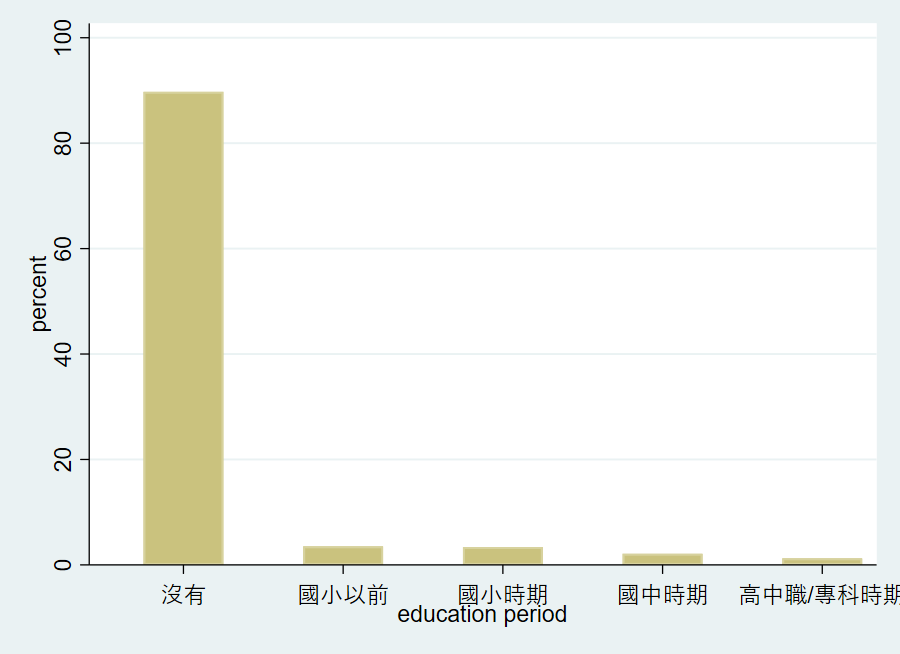
\includegraphics[height=3in]{histogram.png}


\subsection*{Question 4.2}

We use two-way graph to discuss the relationship between $\textit{divorce}$ and $\textit{undergraduate}$, that is, whether encountering divorce reduces the probability of obtaining educational degree higher than undergraduate.

\begin{lstlisting}
recode sh09v33 (9/99 = .)
gen undergraduate = 1 if (sh09v33>=5) & (sh09v33 != .)
replace undergraduate = 0 if (sh09v33<5) & (sh09v33 != .)
twoway (lfit undergraduate divorse)
\end{lstlisting}
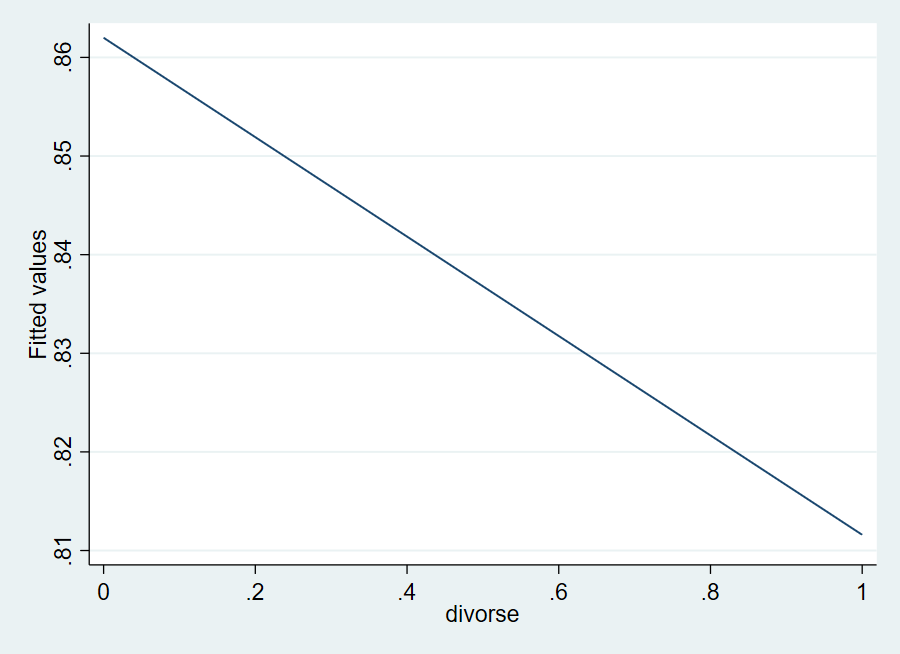
\includegraphics[height=3in]{twoway.png}


\section{Prelimilary Analysis}

\subsection*{Question 5.1}

We can regress the $\textit{undergraduate}$ on $\textit{divorce}$

\begin{lstlisting}
reg undergraduate divorce, r
\end{lstlisting}
The coefficient of $\textit{divorce}$ is negative, which means students in single parent families tend to have less human capital accumulation. This might influence their future performance and wages.


\subsection*{Question 5.2}

Consider the OVB formula 
\[
    \hat{\alpha} \to \alpha + \beta\frac{ Cov (X_i,D_i)}{ \textit{Var} (D_i)}
\]
Since the children in the single parent family might have less economic situation or oppotunity to accumulate their human capital, the correlation is non-zero and thus confounding the outcome.


\subsection*{Question 5.3}

We include other two variables as the control variable, which are the education background of both father and mother.

\begin{lstlisting}
rename _merge merge_2009
merge 1:1 stud_id using "SH/SH_2001_G_parent.dta"
recode w1faedu (6/99 = .)
recode w1moedu (6/99 = .)
gen fa_undergraduate = 1 if (w1faedu>=3) & (w1faedu<=5) & (w1faedu != .)
replace fa_undergraduate = 0 if (w1faedu<3 | w1faedu>5) & (w1faedu != .)
gen ma_undergraduate = 1 if (w1moedu>=3) & (w1moedu<=5) & (w1moedu != .)
replace ma_undergraduate = 0 if (w1moedu<3 | w1moedu>5) & (w1moedu != .)

reg undergraduate divorce fa_undergraduate ma_undergraduate, r
\end{lstlisting}

Since parent's divorce took place after they got the educational degree, with utilizing the panel data, we can verify that the educational status should not be a confounding factor and can control for the causal inference.

\end{document}
